% !Mode:: "TeX:UTF-8"

\chapter{实验设计与分析}
\label{ch:exp}

本章将利用常见的社会关系理解的数据集对上一章提到的PPRN模型进行检测任务的验证,具体来说即对图片中两个标定的坐标人的关系类别。本章首先介绍当前所用到的两个数据集训练/验证/测试的数据分布情况,数据集的特点。再介绍若干对比模型,介绍实验的参数设置,然后分别对实验结果进行说明和分析,并且对其中消息池化进行了不同实现方法的对比。最后通过案例研究的方法来分析PPRN模型在关系补全任务中发挥的效果。

\section{数据集}

\subsection{数据集简介}

现有的大规模社会关系理解的数据集主要有两个:分别是PIPA-relation\cite{sun2017a}数据集和PISC\cite{li2017dual-glance}数据集,下面简单介绍这两个数据集。

PISC数据集全称是People in social Context,它是Sun等人在2017年通过人工标注平台得到的数据集,这些图片主要来自Visual Genome\cite{krishna2017visual}、COCO\cite{lin2014microsoft}、YFCC100M\cite{thomee2016yfcc100m}、instagram 和twitter等社交网站,Google和Bing商业搜索引擎。从这数据额的来源可以保证数据集的图片是足够高的方差的,人的面部表情,以及场景类型。PISC数据集包含22670张图片以及对应的社会关系标注,在PISC数据集上,又包含两个粒度的识别任务,coarse-level和fine-level。如图\ref{fig:exp-pisc-r}所示的划分方式,先是粗粒度的,再到细粒度的关系类别。
\begin{figure}[htpb]
	\centering
	%	\includegraphics[width=0.48 \textwidth, trim=10 10 10 80,clip]{./pic/example_new.pdf}
	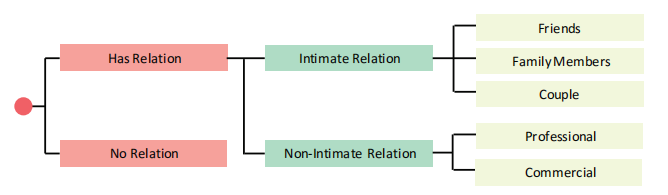
\includegraphics[width=0.98 \textwidth,clip]{pisc-split.png}
	%\hspace{0.02\textwidth}
	%\vspace*{-0.08cm}
    \caption{PISC的关系划分}
	\vspace*{-3.5mm}
	\label{fig:exp-pisc-r}
\end{figure}

PIPA-relation数据集的全称是People in Photo Album Relation,总共包括37107张图片。同样是人工标注的数据集,基于社会关系理论\cite{bugental2000acquisition}划分的,Sun\cite{sun2017a}详细的给出了每个关系域的特征。然后所有的社会关系划分为5个关系域,在构建数据集的过程中,这5个关系域划分为16种社会关系,五个关系域分别是Attachment domain、Reciprocity domain、Mating domain、Hierarchical power domain和Coalitional groups domain。Attach domain划分为father-child,mother-child,Grandpa-grandchild和grandma-grandchild,Reciprocity domain划分为friends, siblings和classmates。Mating domain只包含单条关系lovers/spouses。Hierarchical power domain划分为presenter-audience, teacher-student, trainer-trainee and leader-subordinate。Coalitional groups domain划分为band members, dance team members, sport team members and colleagues。

数据集的情况如表\ref{tab:exp-pisc-statistic},``Train''表示训练集图片的数量,``Valid''和``Test''分别表示验证和测试集的图片数量。``\#train''表示训练集人对的数量,``\#valid''和``\#test''分别表示验证和测试集的人对数量。
\begin{table}[htpb]
  \centering
  \caption{PISC、PIPA-relation数据集的统计列表}
  \setlength{\tabcolsep}{4.5mm}
  \label{tab:exp-pisc-statistic}
  \begin{tabular}{c|c|c|c|c|c|c}
    \toprule
    数据集 & Train & Valid & Test & \#train  &  \#valid &  \#test  \\
    \midrule
    PISC-coarse & 13142 & 4000 & 4000 & 14536 & 25636 & 15497   \\
    \midrule
    PISC-fine &  16828 & 500 & 1250 & 55400 & 1505 & 3691 \\
    \midrule
    PIPA-relation & 5857 & 261 & 2452 & 13729 & 709 & 5106 \\
    \bottomrule
  \end{tabular}
\end{table}

\subsection{数据集分析}

对于数据集PISC-coarse、PISC-fine和PIPA-relation,本文做了基本的数据集分析,如表\ref{tab:exp-data-analysis-1},其中``Sui''表示一张图片有多个人对的比例,``Unsui''则表示一张图片只有一个人对的百分比。·``Single Rel''一张图片包含的关系类别只有一种,``Multi Rel''表示一张图片包含多种关系。从表统计数据可以得到两个结论,从``Sui''和``Unsui''来看,绝大多数的图片是包含多个人对的,从``Multi Rel''来看,一张图片的关系种类往往是相同的,因为直观来看,给定场景下的社会关系时稳定的。例如,假如张图片是一个会议的场景,那么其中往往会有多个人对,并且这些人对间的社会关系往往是``
colleagues''或``presenter audience''。
\begin{table}[htpb]
  \centering
  \caption{PISC 和 PIPA-relation统计分析}
  \label{tab:exp-data-analysis-1}
  \begin{tabular}{c|c|p{0.9cm}<{\centering}|p{0.9cm}<{\centering}||p{0.9cm}<{\centering}|p{0.9cm}<{\centering}}
    \midrule
    \multicolumn{2}{c|}{Dataset} & Sui. & Unsui. & \tabincell{c}{Single\\Rel.} & \tabincell{c}{Multi\\Rel.} \\
    \midrule
    \multirow{2}*{PISC} & coarse & 87.1 & 12.9 & 79.9 & 20.1\\
    \cline{2-6}
    ~ & fine & 83.9 & 16.1 & 86.4 & 13.6 \\
    \midrule
    \multicolumn{2}{c|}{PIPA-relation 16} & 71.9 & 28.1 & 94.9 & 5.1 \\
    \midrule
  \end{tabular}
\end{table}

此外,对于关系类别这项统计,本文做了进一步工作,并且发现一张图片的关系种类大多只是一种,少部分是两种。如图\ref{fig:exp-statistic}所示,在PISC-coarse中,大约79.9\%的图片是只有一种关系类别,20.0\%的图片有含有两个关系。

\begin{figure}[htpb]
	\centering
	%	\includegraphics[width=0.48 \textwidth, trim=10 10 10 80,clip]{./pic/example_new.pdf}
	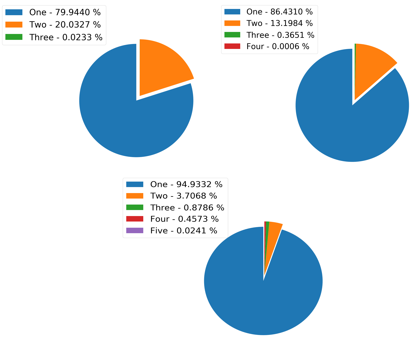
\includegraphics[width=0.65 \textwidth,clip]{ppp.png}
	%\hspace{0.02\textwidth}
	%\vspace*{-0.08cm}
    \caption{数据集的关系类别统计}
	\vspace*{-3.5mm}
	\label{fig:exp-statistic}
\end{figure}

\section{实验设置}

在预训练模型,包括ResNet-101和Vgg-16最后一层的维度都是是4096,经过全连接层,在消息传递和池化模块的中的编码长度为512。池化模块中注意力机制的attention_size=30,结合周边物体信息模块中注意力机制的attention_size=30


\section{实验对比}


